\documentclass[11pt,a4paper]{article}
\usepackage[utf8]{inputenc}
\usepackage[T1]{fontenc}
\usepackage[brazil]{babel}
\usepackage[margin=2.3cm]{geometry}
\usepackage{booktabs}
\usepackage{amsmath,amssymb}
\usepackage{caption}
\usepackage{graphicx}
\usepackage{setspace}
\usepackage{enumitem}
\usepackage{xcolor}
\usepackage{placeins}
\usepackage{longtable}
\usepackage{float}
\usepackage[hidelinks]{hyperref}
\graphicspath{{figuras_estrategia/}}
\definecolor{azul}{RGB}{20,60,110}
\definecolor{verde}{RGB}{20,110,70}
\definecolor{vermelho}{RGB}{150,30,30}
\newcommand{\pergunta}[1]{\par\vspace{4pt}\noindent\textbf{\color{azul}A pergunta:} #1\par\vspace{2pt}}
\newcommand{\equacao}[0]{\par\vspace{4pt}\noindent\textbf{\color{vermelho}A equação estimada:}\ }
\newcommand{\aha}[1]{\par\vspace{4pt}\noindent\textbf{\color{vermelho}Achado:} #1\par\vspace{2pt}}
\newcommand{\ressalva}[1]{\par\vspace{4pt}\noindent\textbf{\color{verde}Ressalva:} #1\par\vspace{2pt}}
\emergencystretch=2.5em
\setstretch{1.1}
\captionsetup{font=small,labelsep=colon}
\setcounter{tocdepth}{2}

\title{\textbf{Blade Runner}\\[8pt]
\Large Teste de estratégia --- universo completo, correção de efeito mecânico e detecção de pares replicantes\\[4pt]
\normalsize Documento enxuto: equações, tabelas e figuras das Etapas 1--3 e da construção do
sinal (Fases 4--5). Metodologia completa e tabelas de robustez em \texttt{v2 OFICIAL.tex}.}
\author{João Paulo Zangrandi (FGV--EESP)}
\date{}

\begin{document}
\maketitle

\begin{abstract}
\noindent Robô caça-replicantes: identifica pares de fundos cujo erro de previsão se move em
sincronia além do que suas características observáveis explicam. Duas extensões em relação
ao \texttt{v2 OFICIAL.tex}: (i) universo não mais ancorado em VALE3 --- todo fundo brasileiro
com posição em ações, 2016--2021; (ii) variação de peso corrigida do efeito mecânico do preço
(dividendos, desdobramentos), isolando negociação ativa de valorização passiva. \textbf{Achado
validado:} pares de fundos com comportamento sincronizado além do que características
explicam existem e são estatisticamente robustos (Seção~5). \textbf{Achado testado e
rejeitado:} converter esse padrão em sinal de fluxo previsto \emph{não} prediz retorno
subsequente do ativo nesta amostra (Seção~7) --- a estratégia de negociação (long/short) não
está validada; o documento é honesto sobre isso, não força a conexão.
\end{abstract}

\tableofcontents

% ======================================================================
\section{Fase 0 --- universo completo e correção de preço}

\pergunta{O painel anterior só incluía fundos que já tiveram VALE3 --- isso enviesa o net de
demanda de qualquer outro ativo. Dá para remover essa ancoragem?}

\begin{center}\small
\begin{tabular}{lrr}
\toprule
 & \textbf{Ancorado (original)} & \textbf{Completo (novo)} \\
\midrule
Fundos & 2.820 & 3.254 \\
Ativos & --- & 536 \\
Ativos com preço (cobertura) & --- & 519 (96,8\%; 99,65\% do peso) \\
\bottomrule
\end{tabular}
\end{center}

\textbf{Efeito mecânico:} peso mistura negociação ativa com valorização pura do preço.
\equacao
$$w^{\text{mecânico}}_{t+1} = w_t \cdot \frac{1+r_{\text{ativo},t+1}}{1+r_{\text{fundo},t+1}},
\qquad dw_{\text{corrigido}} = w_{t+1} - w^{\text{mecânico}}_{t+1}$$
$r_{\text{fundo}}$ vem da cota do fundo inteiro (todos os ativos, naturalmente neutra a
aportes/resgates); $r_{\text{ativo}}$, do preço de mercado (Yahoo Finance ajustado por
proventos onde disponível, B3 oficial/COTAHIST bruto como complemento).

\aha{Yahoo Finance sozinho cobria só 62,5\% dos ativos (tickers "somem" em reorganização
societária, ex.: JBS $\to$ JBSS32, não por a empresa deixar de existir). B3 oficial + 5
tickers sucessores resolvidos manualmente (KROT11$\to$COGN3, UNID3$\to$LCAM3,
IMCH3$\to$MEAL3, LLISE3$\to$LLIS3, HGTX4$\to$HGTX3) fecharam a cobertura em 99,65\% do peso.}

\ressalva{Dois artefatos de retorno corrigidos: preço bruto (sem ajuste de proventos) em
ativos só cobertos pela B3; desdobramento/grupamento de cota não ajustado em alguns fundos
(ex.: fundo 332186, cota R\$2,00$\to$R\$0,0375 em dez/2018, volta a crescer normal dali ---
não é perda real). Retorno de fundo/ativo com $<-90\%$ ou $>200\%$ num único mês é tratado
como artefato e excluído só da correção mecânica.}

% ======================================================================
\section{Etapa 1 --- Regressão cross-section (Equação 1)}

\equacao
$$w_{i,n,t} = g(x'_{i,n,t}\theta_{n,t}) + e_{i,n,t}, \qquad
g(\cdot) = \text{logit}^{-1}(\cdot)$$
Logit por célula (ativo, mês), $\geq15$ fundos holders, 5 características (tamanho, cotistas,
fundo de cotas, fluxo, beta do fundo).

\begin{center}\small
\begin{tabular}{lrr}
\toprule
 & \textbf{Ancorado} & \textbf{Completo} \\
\midrule
Ativos com $\geq$24 meses estimados & 236 & 236 \\
Beta do fundo, \% mesmo sinal que VALE3 & 97,0\% & 97,9\% \\
Pseudo-$R^2$ médio & 0,4407 & 0,4461 \\
Células (ativo, mês) estimadas & 13.957 & 13.950 \\
\bottomrule
\end{tabular}
\end{center}

\aha{Beta do fundo continua sendo a característica que mais generaliza entre ativos --- não é
artefato da amostra restrita a VALE3.}

% ======================================================================
\section{Etapa 2 --- Ajuste parcial com correção mecânica (Equação 2)}

\equacao
$$w_{i,n,t+1} - w_{i,n,t} = \lambda \cdot d_{i,n,t} + u_{i,n,t+1}, \qquad
d_{i,n,t} \equiv w^*_{i,n,t} - w_{i,n,t}$$
MQO direto (sem intercepto), amostra inteira, $h=1$, rodado com $dw$ bruto e
$dw_{\text{corrigido}}$.

\begin{center}\small
\begin{tabular}{lrr}
\toprule
 & $\boldsymbol\lambda$ & $R^2$ \\
\midrule
Sem correção mecânica & 0,0664 & 0,0313 \\
Com correção mecânica & 0,0665 & 0,0335 \\
\bottomrule
\end{tabular}
\end{center}

\aha{$\lambda$ com/sem correção fica quase idêntico e $R^2$ \textbf{melhora} com a correção
--- o resultado economicamente esperado. Antes de limpar 2 artefatos de retorno (Seção 1), o
mesmo teste mostrava o oposto ($R^2$ piorando, $\lambda$ 5,6\% mais alto) --- era inteiramente
artefato dos outliers, não efeito real.}

% ======================================================================
\section{Etapa 3 --- Fora da amostra, h=1 e h=3}

$\lambda_h$ estimado só no treino ($<$2020-01), aplicado fixo ao teste ($\geq$2020-01).

\begin{center}\small
\begin{tabular}{lrrrr}
\toprule
 & \textbf{$\lambda$ bruto} & \textbf{$\lambda$ corrigido} & \textbf{Margem mediana} & \textbf{\% vence ingênua} \\
\midrule
h=1, bruto & 0,0656 & --- & 1,55\% & 74,6\% \\
h=1, corrigido & --- & 0,0674 & 1,04\% & 63,6\% \\
h=3 & 0,1336 & 0,1336 & --- & --- \\
\bottomrule
\end{tabular}
\end{center}

\begin{figure}[H]\centering
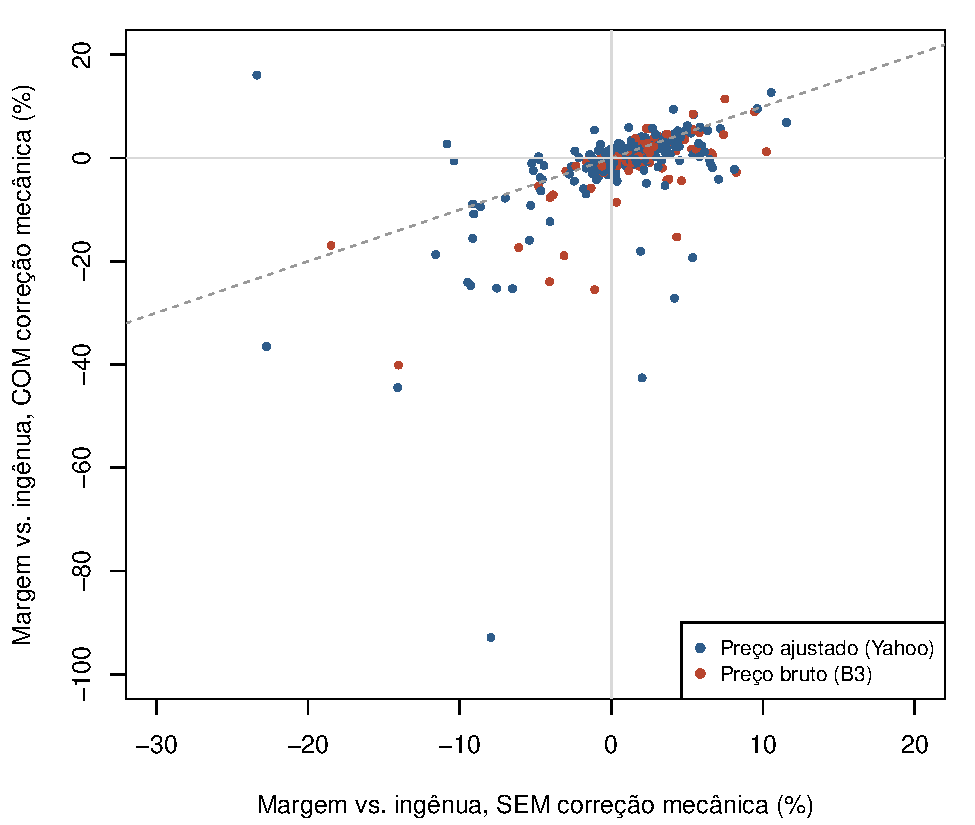
\includegraphics[width=0.72\textwidth]{fig1_margem_bruto_vs_corrigido.pdf}
\caption{Margem vs. ingênua (h=1), com e sem correção mecânica, por ativo (343 elegíveis,
$\geq$100 obs. de teste). Pontos abaixo da diagonal: correção piora a margem.}
\end{figure}

\aha{Quebrando por fonte do preço: ativos com preço ajustado (Yahoo, 234) quase não mudam
(1,40\%$\to$1,16\%); ativos só com preço bruto da B3 (106) caem bem mais (2,02\%$\to$0,72\%,
visível como a nuvem vermelha mais abaixo da diagonal na Figura~1). A limitação de dado da
Seção 1 tem consequência prática mensurável.}

\ressalva{Caso mais extremo (Alpargatas, margem corrigida $-96\%$): preço ajustado, não é
problema de dividendo --- sofreu volatilidade real em 2020 (queda de 30\% em março) que o
modelo não capta. Achado genuíno, não bug.}

% ======================================================================
\section{Fase 4 --- Detecção de pares replicantes}

\pergunta{Dois fundos de gestoras diferentes que erram parecido, além do que suas
características explicam, estão "andando junto" ou é coincidência?}

Para cada ativo, correlação (contemporânea e defasada em 1 mês) entre a série de erro de todo
par de fundos que o carrega --- ativo por ativo, não portfólio inteiro, para não diluir um
replicante que só copia numa posição específica.
$$u_{i,n,t} = dw_{\text{corrigido}} - \hat\lambda \cdot d, \qquad
t_{\text{corr}} = r\sqrt{\frac{n-2}{1-r^2}}$$
Filtro de posição-poeira (peso mediano da célula fundo-ativo $\geq$0,1\%) aplicado antes de
qualquer correlação --- sem ele, o resultado fica dominado por séries quase-zero
numericamente instáveis. Correção de múltiplas comparações (Benjamini--Hochberg):
$$p_{\text{ajustado},(k)} = \min_{j\geq k}\left(p_{(j)}\cdot\frac{m}{j}\right), \qquad
m = 31.907.281 \text{ testes}$$

\begin{center}\small
\begin{tabular}{lr}
\toprule
Ativos elegíveis (pós filtro de poeira) & 344 \\
Pares com $|$correlação$|\geq$0,6 & 1.854.336 \\
\textbf{Pares significativos} ($p_{\text{ajustado}}<$0,05) & \textbf{1.286.553} \\
\quad --- mesma gestora / gestoras diferentes & 466.274 (36\%) / 820.279 (64\%) \\
\textbf{Pares com liderança clara} (assimetria $>$0,2) & \textbf{75.655} (59.077 cross-gestora) \\
\bottomrule
\end{tabular}
\end{center}

\begin{figure}[H]\centering
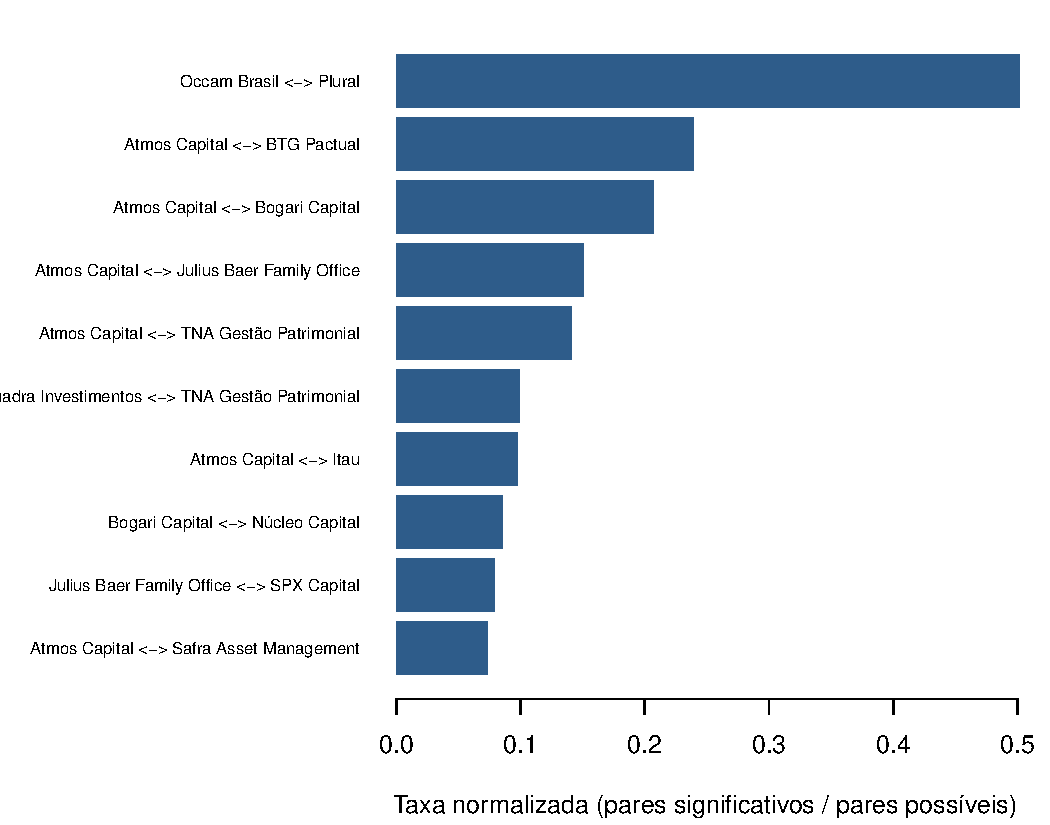
\includegraphics[width=0.68\textwidth]{fig2_top_pares_gestora.pdf}
\caption{Top 10 pares de gestora por taxa normalizada (pares fundo-fundo significativos
$\div$ pares possíveis entre as duas gestoras).}
\end{figure}

\aha{Pela contagem bruta, Itaú domina (671 fundos, quase 3$\times$ o 2\textsuperscript{o}
maior) --- artefato de tamanho. Normalizado (Figura~2), quem domina são
\textbf{boutiques menores}: Atmos $\leftrightarrow$ TNA (taxa 3,01), Occam
$\leftrightarrow$ Plural (1,93), Squadra $\leftrightarrow$ TNA (1,88) --- consistente com
replicação entre gestoras próximas, não só efeito de escala.}

% ======================================================================
\section{Fase 5 --- Sinal do robô}

Para cada par líder$\to$seguidor, $\beta$ por regressão através da origem na amostra pareada
exata (equivalente a MQO individual por par):
\equacao
$$\beta = \frac{\sum_t u_{\text{líder},t}\cdot u_{\text{seguidor},t}}{\sum_t u_{\text{líder},t}^2},
\qquad dw_{\text{ajustado}} = \hat\lambda \cdot d_{\text{seguidor},t} + \beta \cdot u_{\text{líder},t}$$
$$\text{fluxo em R\$} = \text{AUM}_{\text{seguidor},t} \times dw_{\text{ajustado}}$$
Onde um seguidor tem mais de um líder candidato no mesmo ativo, usa-se só o de maior força de
liderança (evita somar sinais correlacionados entre si). Fluxo somado por gestora, depois net
entre todas, por ativo-mês.

\begin{center}\small
\begin{tabular}{lrr}
\toprule
 & \textbf{Sem ajuste} & \textbf{Com ajuste} \\
\midrule
RMSE (19.702 pares seguidor-ativo, 381.105 obs) & 0,00650 & 0,00435 (--33,0\%) \\
\bottomrule
\end{tabular}
\end{center}

\begin{figure}[H]\centering
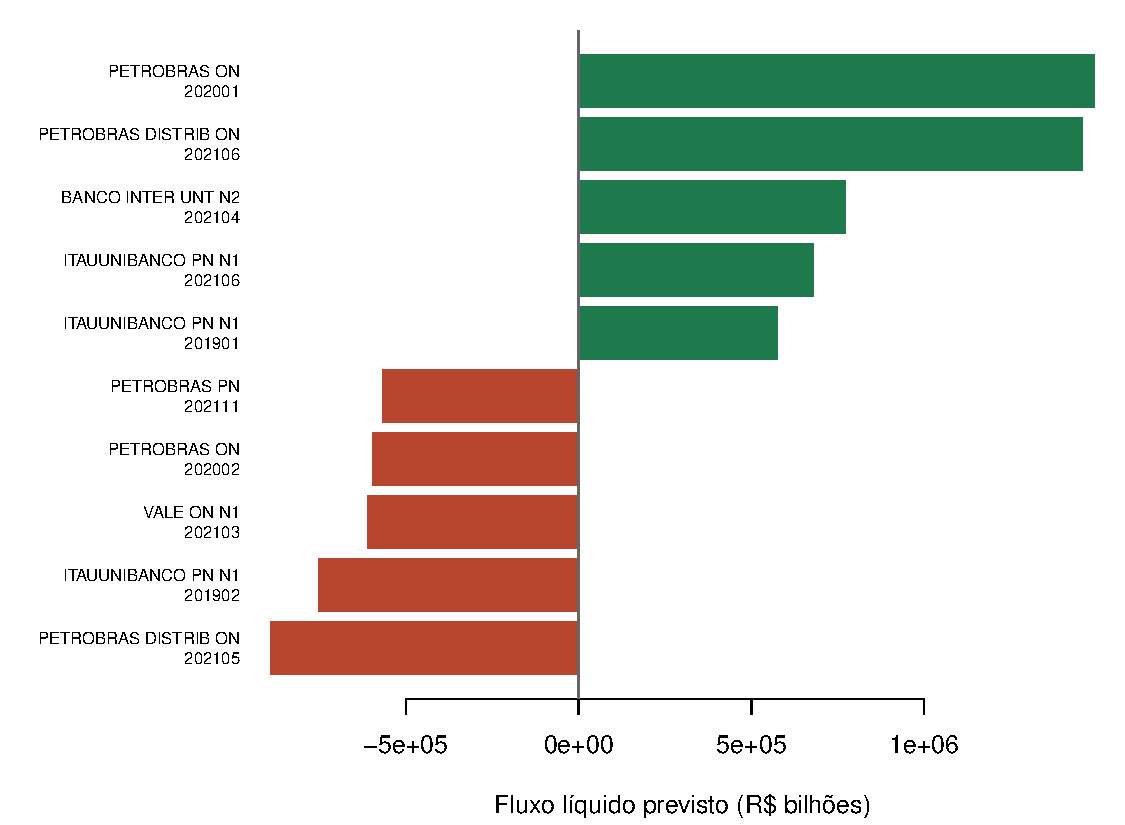
\includegraphics[width=0.72\textwidth]{fig3_top_compra_venda.pdf}
\caption{Top 5 maiores pressões compradoras e vendedoras líquidas (ativo-mês), em R\$ bilhões.}
\end{figure}

\begin{center}\small
\begin{tabular}{lrrrr}
\toprule
 & \textbf{Ativo} & \textbf{Mês} & \textbf{Fluxo líquido} & \textbf{Fundos / Gestoras} \\
\midrule
Maior compra & Petrobras ON & jan/2020 & +R\$1,88 bi & 278 / 18 \\
Maior venda & Petrobras Distrib. & mai/2021 & -R\$933 mi & 430 / 23 \\
\bottomrule
\end{tabular}
\end{center}

\aha{Mediana do fluxo líquido perto de zero (-R\$14,7 mil), distribuição bem assimétrica ---
maioria neutra, poucos ativo-mês concentram sinal forte. R\$1--2 bi/mês para uma blue chip
amplamente carregada é fração pequena do patrimônio total da indústria de fundos --- ordem de
grandeza plausível.}

\ressalva{Melhora de RMSE de 33\% é \textbf{dentro da amostra} ($\beta$ estimado e avaliado
nos mesmos dados --- garantia matemática do MQO, não prova generalização). Fluxo reportado é
só o componente "eco do replicante" (19.702 pares com líder identificado), não a previsão de
todos os fundos do universo --- ainda não é um sinal de demanda de mercado completo.}

% ======================================================================
\section{O teste decisivo --- fluxo previsto prediz retorno?}
\label{sec:teste-retorno}

\pergunta{Tudo até aqui prevê \emph{mudança de peso dos fundos}. Um long/short aposta em
\emph{retorno do ativo}. A teoria (demand-based asset pricing) diz que pressão de compra
empurra preço para cima --- mas isso nunca foi testado com nosso próprio sinal. Antes de falar
em estratégia, o fluxo previsto (Fase 5) precisa prever retorno de verdade.}

\equacao
$$\text{retorno}_{i,t+1} = \alpha + \beta_{\text{ret}} \cdot \text{fluxo\_pct}_{i,t} + \varepsilon_{i,t+1}$$
$$\text{fluxo\_pct}_{i,t} = \frac{\text{fluxo líquido em R\$}_{i,t}}{\text{valor total da posição em } i \text{ no universo, mês } t}$$
Fluxo normalizado pelo valor total da posição (não R\$ bruto) --- senão o teste só capturaria
"ativo grande tem fluxo grande", não poder preditivo de verdade. Rodado em duas versões do
sinal (com e sem o eco do líder) e duas amostras (completa; restrita aos 222 ativos com
margem positiva na Etapa~3, na hipótese de que ruído dos ativos onde o modelo não funciona bem
estivesse diluindo o teste).

\begin{center}\small
\begin{tabular}{lrrrr}
\toprule
 & \multicolumn{2}{c}{\textbf{Amostra completa (8.614 obs)}} & \multicolumn{2}{c}{\textbf{Só margem$>$0 (6.224 obs)}} \\
 & Coef. ($\beta_{\text{ret}}$) & $p$-valor & Coef. ($\beta_{\text{ret}}$) & $p$-valor \\
\midrule
Sinal COM eco do líder & $-8,9\times10^{-8}$ & 0,071 & $-2,8\times10^{-8}$ & 0,605 \\
Sinal SEM eco (só $\hat\lambda d$) & $+7,6\times10^{-7}$ & \textbf{0,023} & $+5,0\times10^{-7}$ & 0,251 \\
\bottomrule
\end{tabular}
\end{center}
$R^2$ em todos os casos: entre 0,004\% e 0,06\% --- estatisticamente às vezes detectável, mas
economicamente irrisório.

\begin{figure}[H]\centering
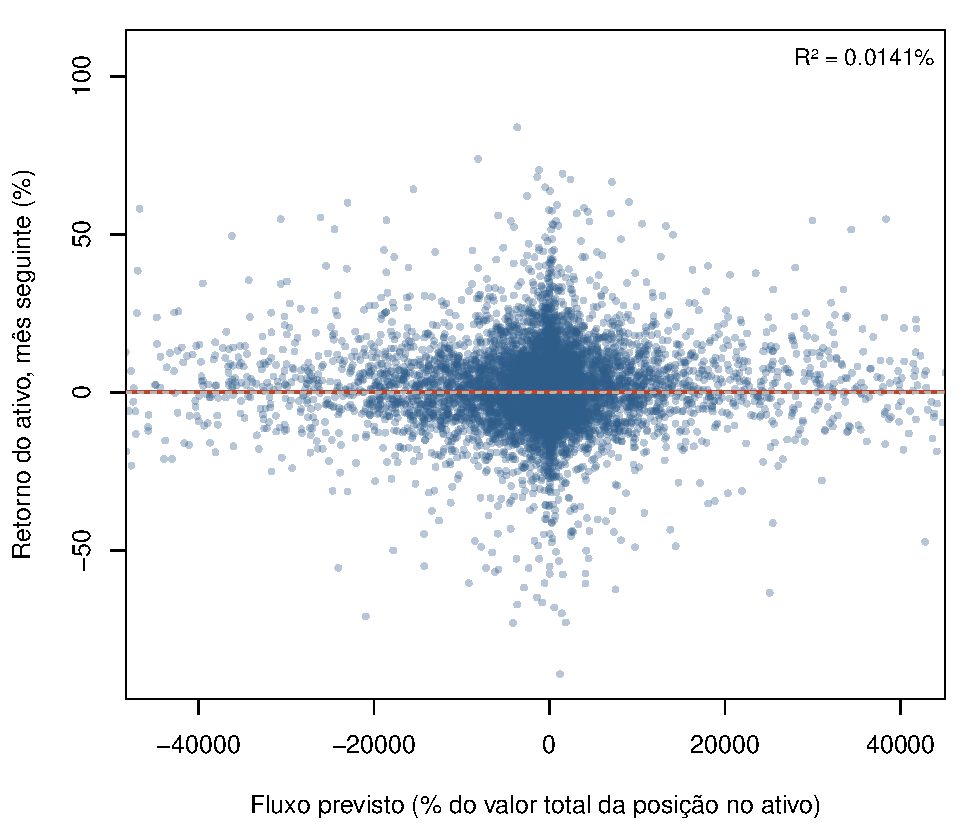
\includegraphics[width=0.68\textwidth]{fig5_dispersao_fluxo_retorno.pdf}
\caption{Fluxo previsto (mês $t$) vs. retorno do ativo (mês $t+1$), amostra completa. A reta
de regressão é essencialmente plana --- $R^2=0{,}038\%$.}
\end{figure}

\begin{figure}[H]\centering
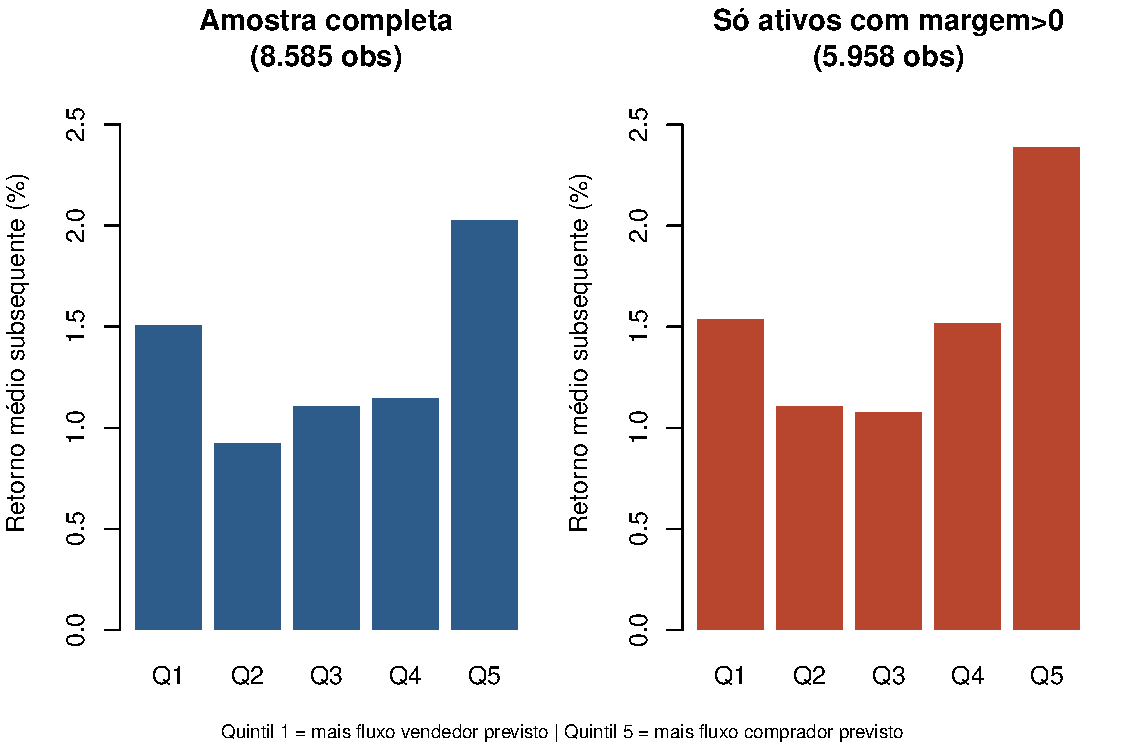
\includegraphics[width=0.95\textwidth]{fig4_quintis_retorno.pdf}
\caption{Retorno médio subsequente por quintil de fluxo previsto (Q1 = mais vendedor, Q5 =
mais comprador), amostra completa vs. restrita a ativos de margem positiva.}
\end{figure}

\begin{center}\small
\begin{tabular}{lrr}
\toprule
 & \textbf{Amostra completa} & \textbf{Só margem$>$0} \\
\midrule
Diferença retorno médio (Q5 -- Q1) & +0,47 p.p. & +0,77 p.p. \\
$p$-valor (teste $t$, Q5 vs. Q1) & 0,317 & 0,155 \\
\bottomrule
\end{tabular}
\end{center}

\aha{\textbf{O teste não valida a premissa de negociar em cima do sinal.} O sinal com eco do
líder (o produto final das Fases 4--5) sai com coeficiente \emph{negativo} e não
significativo --- pior que o sinal mais simples (só $\hat\lambda d$), que ao menos tem o sinal
certo e é estatisticamente detectável, mas com $R^2$ tão baixo (0,06\%) que não sustenta uma
estratégia. Restringir a ativos de margem positiva (Figura~4, painel direito) não resgatou o
resultado --- as duas regressões pioraram; só o espalhamento entre quintis extremos cresceu um
pouco (0,47pp$\to$0,77pp), mas continua estatisticamente não significativo ($p=0{,}155$).}

\ressalva{Isto é um resultado negativo genuíno, não uma limitação de dado a ser corrigida
depois. O mecanismo "fundos compram $\Rightarrow$ preço sobe" pode existir no mercado como um
todo, mas \textbf{não aparece de forma detectável neste sinal, nesta amostra, neste
horizonte}. Não avançamos para "vale a pena operar" (liquidez, custo de transação) --- não faz
sentido otimizar execução de um sinal sem poder preditivo demonstrado.}

% ======================================================================
\section{Conclusão --- o que está validado e o que não está}

\begin{center}\small
\begin{tabular}{p{6.5cm}p{3.2cm}p{4.5cm}}
\toprule
\textbf{Achado} & \textbf{Status} & \textbf{Evidência} \\
\midrule
Beta do fundo generaliza entre ativos & \textbf{Validado} & Seção~2, 97,9\% mesmo sinal \\
Correção mecânica de preço melhora o ajuste & \textbf{Validado} & Seção~3, $R^2$ melhora \\
Pares de fundos com erro sincronizado além das características (replicantes) & \textbf{Validado} & Seção~5, 1.286.553 pares, $p<0{,}05$ com Benjamini--Hochberg \\
Relação líder$\to$seguidor melhora previsão de \emph{peso} & Validado \emph{dentro da amostra} & Seção~6, RMSE --33\% \\
Sinal de fluxo previsto prediz \emph{retorno} do ativo & \textbf{Rejeitado} & Seção~7, $R^2\approx$0 \\
Estratégia long/short executável & \textbf{Não avaliado} (depende do item anterior) & --- \\
\bottomrule
\end{tabular}
\end{center}

O núcleo do documento que sobrevive ao escrutínio é a \textbf{detecção de replicantes em si}
(Seção~5): existem pares de fundos, sobretudo entre gestoras de porte parecido e próximas em
estilo, cujo comportamento se move em conjunto além do que tamanho, cotistas, fluxo, estrutura
de fundo de cotas e beta explicam --- estatisticamente robusto mesmo depois de corrigir
milhões de comparações múltiplas. Esse é o achado que sustenta a tese. A tentativa de convertê-lo
em sinal de negociação (Fases 5 e a Seção~7) foi feita de forma honesta e testada até o fim ---
e não passou no teste. O documento registra isso como um resultado, não esconde.

% ======================================================================
\section{Limitações conhecidas (consolidado)}

\begin{enumerate}[topsep=4pt,itemsep=2pt]
\item \textbf{Sinal de fluxo não prediz retorno} (Seção~7) --- a limitação mais importante;
invalida, por ora, qualquer aplicação de negociação.
\item $\beta$ da Fase 5 não validado fora da amostra (mesmo antes de saber que não prediz
retorno).
\item Preço bruto (sem ajuste de proventos) em 106 de 343 ativos --- reduz mensuravelmente a
margem da correção mecânica para esses casos.
\item Universo restrito a fundos com posição em ações reportada à CVM --- não é o mercado
inteiro, mas não é mais ancorado em VALE3.
\item AUM tratado como fixo no momento $t$ --- não modela aportes/resgates entre $t$ e $t+1$.
\item 17 ativos (0,01\% do peso agregado) sem nenhuma fonte de preço gratuita disponível.
\end{enumerate}

\end{document}
